\documentclass[Deriaz_Traiber_Labo02]{subfiles}


\begin{document}
\chapter{Antenne dipôle}
\section{Objectif}
Le but est de réaliser une antenne qui résonne autour de \SI{2.45}{\giga\hertz}. Le $s_{11}$ à cette fréquence doit être inférieur à \SI{10}{\deci\bel}.


\begin{figure}[H]
\centering
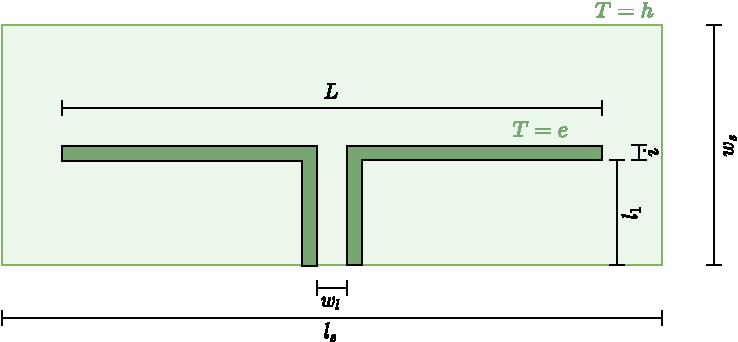
\includegraphics[scale=1,page=1]{../Schemas-crop.pdf}
\caption{Dimensions de l'antenne dipôle}
\label{fig:Schemas-crop}
\end{figure}
\begin{table}[H]
\centering
\begin{tabular}{lll}
\textbf{Variables}\\\hline
$l_1$ & Hauteur du pied\\
$i$   & Épaisseur des brins\\
$w_s$ & Largeur du PCB & \SI{30}{\milli\meter}\\
$l_s$ & Longueur du PCB & \SI{80}{\milli\meter}\\
$L$   & Longueur de l'antenne\\
\textbf{Constantes} & & \textbf{Valeur}\\\hline
$w_l$ & Espacement entre les brins & \SI{1.7}{\milli\meter}\\
$h$ & Épaisseur du PCB & \SI{1.6}{\milli\meter}\\
$e$ & Épaisseur de cuivre & \SI{35}{\micro\meter}
\end{tabular}
\caption{Liste des dimensions}
\end{table}

%------------------------------------------------------------------------------------------------------------------
%	FR4
%------------------------------------------------------------------------------------------------------------------

\section{FR-4}
La longueur d'un brin horizontal est donnée par l'équation \ref{eq_dipole_longueur}
\begin{equation}
\boxed{L_2 = \dfrac{\lambda}{2 \cdot \sqrt{\varepsilon_r}} = \dfrac{c}{2 \cdot F_r \sqrt{\varepsilon_r}}} \Rightarrow L_2 = \dfrac{3\cdot10^8}{2\cdot2.45\cdot1 0^9\cdot \sqrt{4.3}} = \underline{\underline{\SI{29.5}{\milli\meter}}}
\label{eq_dipole_longueur}
\end{equation}
La dimension du pied est donnée par
\begin{equation}
\boxed{l_1=\frac{\lambda}{8}=\frac{c}{8 \cdot F_r}} = \frac{3\cdot 10^8}{8\cdot 2.45\cdot 10^9} \Rightarrow l_1 = \underline{\underline{\SI{15.3}{\milli\meter}}}
\end{equation}
La largeur des brins ($i$) a été fixée à \SI{0.8}{\milli\meter} pour le moment.
\subsection{Itérations}
\subsubsection{Premières itérations}

Afin de se familiariser avec le dimensionnement de l'antenne dipôle planaire, la méthode utilisé consiste à modifier un seul des paramètres jusqu'à obtenir le résultat le plus proche possible des performances souhaitées puis de réaliser le même démarche pour un second paramètre et ainsi de suite pour les autres paramètres.\\

Afin de mettre en évidence l'influence de chaque paramètre de l'antenne sur ses performances, il a été choisi de premièrement trouver les meilleures performances de $S_{11}$ possible en modifiant uniquement la longueur des brins horizontaux de l'antenne, soit $L_2$. Le paramètre $L_2$ correspond à la \textbf{longueur d'un seul brin horizontal} du dipôle. Le paramètre $L$ illustré sur le schéma de la figure \ref{fig:Schemas-crop} est donc décrit par :
$$
L = 2\cdot L_2 + w_l 	\quad \text{avec} \quad  w_l \ll 2 \cdot L_2  \quad \Rightarrow \quad \boxed{L = 2\cdot L_2}
$$

\pagebreak

\begin{flushleft}
La figure \ref{fig:ant1_FR4_2} illustre les premières itérations du dimensionnement de l'antenne dipôle sur substrat FR4 :
\end{flushleft}
\figc{1}{ant1_FR4_1}{Dimensionnement de l'antenne en ne variant que $L$}

\begin{flushleft}
	La figure \ref{fig:ant1_FR4_2} permet de constater plusieurs points intéressants :
\end{flushleft}
\begin{description}
\item \textbf{Premièrement}, il ressort nettement sur les courbes de $S_{11}$, obtenues par simulation, que l'antenne possède deux modes résonants dans la plage de simulation définie ($0\dots$\SI{4}{\giga\hertz}), typiquement \SI{1.2}{\giga\hertz} et \SI{2.75}{\giga\hertz} pour $L_2 = \SI{38}{\milli\meter}$. Ces modes résonnants sont simplement dues à la géométrie en "\textit{équerre}" de l'antenne dipôle.\\
Il ressort aussi que les fréquences des modes résonnants de l'antenne sont inversement proportionnelles à la longueur du brin. Plus simplement, une diminution de la longueur du brin horizontal à pour conséquence de "\textit{pousser}" les modes (pics de résonance) vers la droite et inversement. Ce qui est logique, car il a été mis en évidence, dans la théorie, que la longueur des brins horizontaux était liée à la fréquence de résonance par la relation  $L_2 = c/(2\cdot F_r \cdot \sqrt{\varepsilon_r})$. Une augmentation de la fréquence de résonance à donc bien pour conséquence une diminution de la longueur de $L_2$ et réciproquement.\\

\item \textbf{Deuxièmement}, la longueur de brin $L_2$ calculée dans la théorie ne donne pas les résultats escomptés. Typiquement, une longueur de brin, $L_2=29.5\si{\milli\meter}$, donne deux modes résonnants, soit \SI{1.412}{\giga\hertz} et \SI{3.044}{\giga\hertz}, ce qui est très éloigné de la fréquence de résonance $F_r=\SI{2.45}{\giga\hertz}$ souhaitée.\\

\item \textbf{Troisièmement}, lorsque la longueur de brins $L_2$ diminue et donc que la fréquence de résonance des modes augmente, il apparait que la valeur du $S_{11}$ diminue rapidement pour le premier mode résonnant.\\
\end{description}

\pagebreak

Une fois la meilleure valeur de $L$ déterminée, ici $L_2 = \SI{38}{\milli\meter}$, il est ensuite nécessaire d'améliorer les performances de l'antenne en variant cette fois la longueur du pied de l'antenne ($l_1$) et cela en gardant la longueur $L_2$ déterminée à l'étape précédente.\\

La figure \ref{fig:ant1_FR4_2} illustre le dimensionnement de la longueur du pied de l'antenne ($l_1$) afin d'obtenir le meilleur $S_{11}$ possible pour la fréquence souhaitée de \SI{2.45}{\giga\hertz} :

\figc{1}{ant1_FR4_2}{Dimensionnement de l'antenne en variant que $l_1$}


\begin{flushleft}
	La figure \ref{fig:ant1_FR4_2} permet de constater plusieurs points intéressants :
\end{flushleft}
\begin{description}
\item \textbf{Premièrement}, il apparait clairement que la longueur proposée par la théorie, soit $l_1=\lambda/2$ ne donne pas du tout les meilleures performances.\\

\item \textbf{Deuxièmement}, lorsque la longueur du pied de l'antenne ($l_1$) varie, cela influe sur deux paramètres ; la fréquence de résonance du mode et sa valeur de $S_{11}$. Il semble par contre que l'influence sur la fréquence du mode est moins prononcée que celle due à la longueur des brins horizontaux ($L_2$). De plus, l'influence est encore plus faible pour le premier mode que pour le second, ce qui nous arrange.\\

\item \textbf{Troisièmement}, La meilleure valeur de $S_{11}$ est obtenu avec la longueur de pied d'antenne $l_1$ la plus faible. Il faudra donc chercher à diminuer cette valeur au maximum.
\end{description}

Ce procédé a été réalisé jusqu'à obtenir un résultat satisfaisant par rapport à l'objectif fixé dans la première partie, soit un $S_{11}$ inférieur à \SI{-10}{\decibel}. Les valeurs de paramètres trouvés en ne variant que $L_2$ et $l_1$ donnant des performances satisfaisantes est :
\begin{table}[H]
\centering
\begin{tabular}{c c c}
$\boxed{L_2 = \SI{21}{\milli\meter}}$ & et &  $\boxed{l_1 = \SI{0.5}{\milli\meter}}$
\end{tabular}
\end{table}

\pagebreak

\subsection{Balayage des paramètres variables}

Maintenant que les paramètres principaux de l'antenne ont été grossièrement dimensionnés. Il est intéressant de se pencher sur l'influence des autres paramètres encore disponible, soit :
$$
i \text{ : Épaisseur des brins} \quad \quad \quad w_s \text{ : Largeur du PCB} \quad \quad \quad l_s \text{ : Longueur du PCB}
$$

Une méthode intéressante pour comprendre l'influence de chaque paramètre sur les performances de l'antenne consiste à réaliser une suite de simulation en faisant variant chaque paramètre individuellement afin d'en constater l'impacte sur la courbe du $S_{11}$.\\

La figure \ref{fig:bipol_param_sweep_fr4} illustre les différentes courbes de $S_{11}$ obtenues par le balayage de la valeur de chaque paramètre :

\figc{1}{bipol_param_sweep_fr4}{Balayage de paramétrique de l'antenne dipôle avec substrat FR4}

Il apparait de manière évidente sur la figure \ref{fig:bipol_param_sweep_fr4} que certains paramètres ont beaucoup plus d'influence que d'autre sur la courbe du $S_{11}$. Il ressort même que deux courbes ont été décalés de \SI{250}{\mega\hertz} de part est d'autre de la fréquence visée (\SI{2.45}{\giga\hertz}). Les autres courbes restent condensées, proches de la fréquence cible et ne varie que très légèrement.\\

Afin de mieux mettre en évidence l'influence de chaque paramètre sur les différents critères de performance de l'antenne, il est intéressant d'illustrer la variation normalisée de chaque critère de performance par rapport au changement des dits paramètres.\\

\pagebreak

La figure \ref{fig:bipol_param_norm_sweep_fr4} illustre la variation normalisée des critères de performances de l'antenne en fonction du dimensionnement de ses paramètres :

\figc{1}{bipol_param_norm_sweep_fr4}{Variation normalisée des critères de performance}

Il ressort très nettement sur la figure \ref{fig:bipol_param_norm_sweep_fr4}, que certains paramètres ont une influence sur les critères de performance nettement plus marquée que d'autre, il est possible de remarquer les points suivants :\\

\begin{itemize}
\item [\textbf{Larg. de brin }\textcolor{blue}{$i$}  ] : Le paramètre le plus influant sur les trois critères de performances, soit le $S_{11}$, la fréquence de résonance et la bande passante. Une diminution de \SI{10}{\percent} de $i$ engendre une augmentation d'environ \SI{10}{\percent} du de la fréquence de résonance et de la bande passante ainsi qu'une diminution de presque \SI{5}{\percent} du $S_{11}$. Un comportement équivalant, mais de polarité inverse est visible pour une augmentation de \SI{10}{\percent} de $i$.\\

\item [\textbf{Long. de brin vert. }\textcolor{blue}{$l_1$}] : Deuxième paramètre le plus influant. Une diminution de \SI{10}{\percent} de $l_1$ engendre principalement une diminution de presque \SI{5}{\percent} du $S_{11}$. À l'inverse, une augmentation de \SI{10}{\percent} de $l_1$ engendre une augmentation de presque \SI{5}{\percent} du $S_{11}$ et aussi une faible augmentation de presque \SI{2}{\percent} de la bande passante.\\

\item [\textbf{Long. de brin hor.  }\textcolor{blue}{$L_2$}] : Influence assez faiblement les critères de performance de l'antenne. Une augmentation de quelques \si{percent} apparait lorsque la valeur de $L_2$ est augmenté. Sinon une légère augmentation de quelques \si{percent} du $S_{11}$ est visible lorsque $L_2$ diminue de \SI{10}{\percent}.\\ 

\item [\textbf{Long. du PCB }\textcolor{blue}{$l_s$}] : N'influence quasiment que la valeur du $S_{11}$, et cela, de manière non linéaire et avec de faibles variations.\\

\item [\textbf{Larg. du PCB  }\textcolor{blue}{$w_s$}] : N'influence que le $S_{11}$, cela de manière linéaire et inversement proportionnel à la variation de la valeur de $w_s$.\\
\end{itemize}

\pagebreak

La table \ref{tab:param-sweep-fr4} décrit en détail l'influence de chaque paramètre de l'antenne sur les critères de performance de cette dernière :

\begin{table}[H]
\centering
\begin{tabular}{|l|c|cc|cc|cc|c|}\hline
	Var 		   	& ID  &  $S_{11}$ \si{[\decibel]} &  $dS_{11}$ \si{[\percent]}   &  $F_r$ \si{[\giga\hertz]} &   $dF_r$ \si{[\percent]}  & $BW$\si{[\mega\hertz]} &   $dBW$ \si{[\percent]}  \\ \hline\hline
    $  +    \SI{ 0}{\percent}  $ &   1  &   -32.19  &        0   &  2.452  &          0  &   260  &          0\\\hline                                               
    $ i -   \SI{10}{\percent}  $ &   2  &  -30.763  &   -4.4337  &   2.68  &     9.2985  &   292  &     12.308\\                                                         
    $ i -   \SI{ 1}{\percent}  $ &   3  &  -32.095  &  -0.29627  &  2.472  &    0.81566  &   264  &     1.5385\\                                                         
    $ i +   \SI{ 1}{\percent}  $ &   4  &  -32.326  &   0.42274  &  2.428  &   -0.97879  &   260  &          0\\                                                         
    $ i +   \SI{10}{\percent}  $ &   5  &  -33.418  &    3.8133  &  2.256  &    -7.9935  &   236  &    -9.2308\\\hline                                                         
    $ l_1 - \SI{10}{\percent}  $ &   6  &  -30.849  &   -4.1664  &  2.448  &   -0.16313  &   260  &          0\\                                                         
    $ l_1 - \SI{ 1}{\percent}  $ &   7  &  -32.077  &  -0.35265  &  2.452  &          0  &   260  &          0\\                                                         
    $ l_1 + \SI{ 1}{\percent}  $ &   8  &  -32.302  &    0.3489  &  2.452  &          0  &   260  &          0\\                                                         
    $ l_1 + \SI{10}{\percent}  $ &   9  &  -33.309  &    3.4767  &  2.452  &          0  &   264  &     1.5385\\\hline                                                         
    $ L_2 - \SI{10}{\percent}  $ &  10  &  -32.641  &    1.3998  &  2.452  &          0  &   260  &          0\\                                                         
    $ L_2 - \SI{ 1}{\percent}  $ &  11  &  -32.235  &   0.13911  &  2.452  &          0  &   260  &          0\\                                                         
    $ L_2 + \SI{ 1}{\percent}  $ &  12  &  -31.888  &  -0.93852  &  2.448  &   -0.16313  &   256  &    -1.5385\\                                                         
    $ L_2 + \SI{10}{\percent}  $ &  13  &  -32.139  &  -0.15899  &  2.452  &          0  &   260  &          0\\\hline                                                         
    $ l_s - \SI{10}{\percent}  $ &  14  &  -31.693  &   -1.5444  &  2.452  &          0  &   260  &          0\\                                                         
    $ l_s - \SI{ 1}{\percent}  $ &  15  &  -32.207  &  0.051382  &  2.452  &          0  &   260  &          0\\                                                         
    $ l_s + \SI{ 1}{\percent}  $ &  16  &  -32.229  &   0.11976  &  2.452  &          0  &   260  &          0\\                                                         
    \textcolor{blue}{$ l_s + \SI{10}{\percent}$}   & \textcolor{blue}{17} & \textcolor{blue}{-32.621} & 1.3393 & \textcolor{blue}{2.452} & 0 & \textcolor{blue}{264} & 1.5385\\\hline                                                         
    $ w_s - \SI{10}{\percent}  $ &  18  &   -32.83  &    1.9869  &  2.456  &    0.16313  &   260  &          0\\                                                         
    $ w_s - \SI{ 1}{\percent}  $ &  19  &  -32.329  &   0.43203  &  2.452  &          0  &   260  &          0\\                                                         
    $ w_s + \SI{ 1}{\percent}  $ &  20  &  -32.117  &  -0.22786  &  2.448  &   -0.16313  &   260  &          0\\                                                         
    $ w_s + \SI{10}{\percent}  $ &  21  &  -31.623  &   -1.7619  &  2.448  &   -0.16313  &   260  &          0\\\hline            
\end{tabular}
\caption{Table de la variation des performances de l'antenne - FR4}
\label{tab:param-sweep-fr4}
\end{table}

\subsection{Meilleures performances}

Grâce au balayage de valeur des paramètres de l'antenne, il est possible de trouver le meilleur compromis pour obtenir les meilleures performances. Le meilleur candidat sélectionné est la simulation N\textsuperscript{\underline{o}}$17$, dont les paramètres sont décrits dans la table \ref{tab:best-perf-fr4} :

\begin{table}[H]
\centering
\begin{tabular}{||l c c||}    \hline
    ID      &    $17$     &  $-$ \\\hline
     i       &   $0.8$    &  \si{\milli\meter}\\
    $l_1$     &  $0.5$   &   \si{\milli\meter}\\
    $L_2$     & $20.96$  &  \si{\milli\meter}\\
    $l_s$      & $88$     &  \si{\milli\meter}\\
    $w_s$      & $30$     &  \si{\milli\meter}\\\hline
\end{tabular}
     \caption{Paramètre de l'antenne avec les meilleures performances (FR4)}
     \label{tab:best-perf-fr4}
\end{table}

\pagebreak

La figure \ref{fig:bipol_param_sweep_fr4_best} illustre la courbe de $S_{11}$ du candidat de simulation N\textsuperscript{\underline{o}}$17$, soit celui possédant les meilleures performances :

\figc{1}{bipol_param_sweep_fr4_best}{Courbe $S_{11}$ avec les paramètres donnant les meilleures performances générales (FR4)}

L'antenne ainsi dimensionnée remplie bien les objectifs souhaités, car elle possède un $S_{11} = \SI{-33.3}{\decibel}$ et une bande passante à \SI{-10}{\decibel} $\text{BW} = \SI{264}{\mega\hertz}$ ainsi qu'une fréquence de résonance de \SI{2.45}{\giga\hertz}.

\subsection{Rayonnement (champ lointain) avec les meilleures performances}

\figc{0.9}{bipol_farfield_dir_fr4}{Directivité de l'antenne - Céramique}

\begin{table}[H]
\centering
\begin{tabular}{l c}\hline
Type					& Farfield\\
Approximation		& enable($\text{kR}\gg1$)\\
Component			& Abs\\
Output				& Directivity\\
Frequency			& \SI{2.45}{\giga\hertz}\\
Radial Efficacity	& \SI{-0.01015}{\decibel i} $\Rightarrow$ \SI{99.77}{\percent}\\
Total Efficacity		& \SI{-0.01256}{\decibel i} $\Rightarrow$ \SI{99.71}{\percent}\\
Directivity			& \SI{2.421}{\decibel i}\\
Gain	 (IEEE)			& \SI{2.411}{\decibel i}\\
Realized Gain		& \SI{2.408}{\decibel i}\\\hline
\end{tabular}
\end{table}


%------------------------------------------------------------------------------------------------------------------
%	CERAMIQUE
%------------------------------------------------------------------------------------------------------------------

\pagebreak

\section{Céramique}

La méthode de prédimensionnement de l'antenne avec substrat en céramique est similaire à celui réalisé pour l'antenne avec substrat en FR4. Cette étape étant rébarbative, le choix est fait de passer directement au balayage des valeurs de paramètres.

\subsection{Balayage des paramètres variables}


La figure \ref{fig:bipol_param_sweep_alumina} illustre les différentes courbes de $S_{11}$ obtenues par le balayage de la valeur de chaque paramètre:

\figc{1}{bipol_param_sweep_alumina}{Balayage de paramétrique de l'antenne dipôle avec substrat en céramique}

Il apparait de manière évidente sur la figure \ref{fig:bipol_param_sweep_alumina} que certains paramètres ont beaucoup plus d'influence que d'autre sur la courbe du $S_{11}$. Il ressort aussi que deux courbes sont décalées de \SI{250}{\mega\hertz} de part est d'autre de la fréquence visée (\SI{2.45}{\giga\hertz}). Les autres courbes restent condensées, proches de la fréquence cible et ne varie que très légèrement.\\

Comme pour l'antenne avec substrat FR4, il est aussi intéressant d'illustrer la variation normalisée de chaque critère de performance par rapport au changement des dits paramètres.\\

\pagebreak

La figure \ref{fig:bipol_param_norm_sweep_alumina} illustre la variation normalisée des critères de performances de l'antenne en fonction du dimensionnement de ses paramètres :

\figc{1}{bipol_param_norm_sweep_alumina}{Variation normalisée des performances}

Il ressort aussi très nettement sur la figure \ref{fig:bipol_param_norm_sweep_alumina}, que certains paramètres ont une influence sur les critères de performance nettement plus marquée que d'autre, il est possible de remarquer les points suivants :\\

\begin{itemize}
\item [\textbf{Larg. de brin }\textcolor{blue}{$i$}  ] : Le paramètre le plus influant sur les trois critères de performances, soit le $S_{11}$, la fréquence de résonance et la bande passante. Une diminution de \SI{10}{\percent} de $i$ engendre une augmentation de plus de \SI{10}{\percent} de la bande passante et presque de \SI{10}{\percent} pour la fréquence de résonance ainsi qu'une diminution de presque \SI{2}{\percent} du $S_{11}$. Contrairement à l'antenne sur FR4, il n'apparait pas un comportement de polarité inverse équivalent pour une augmentation de \SI{10}{\percent} de $i$. Seul la bande passante semble être significativement impacté par la variation de $i$.\\

\item [\textbf{Long. de brin vert. }\textcolor{blue}{$l_1$}] : Influence quasiment uniquement la bande passante de l'antenne. Une augmentation oscillant entre \SI{2}{\percent} et \SI{4}{\percent} est visible pour toutes les variations de la valeur de $l_1$..\\

\item [\textbf{Long. de brin hor.  }\textcolor{blue}{$L_2$}] : Deuxième paramètre le plus influent sur les performances de l'antenne. Seul une diminution de \SI{10}{\percent} de $L_2$ engendre une diminution d'approximativement \SI{8}{\percent} de la fréquence de résonance et de la bande passante. Sinon, une augmentation quasiment constante d'environ \SI{4}{\percent} est visible pour les autres valeurs de $l_2$.\\

\item [\textbf{Long. du PCB }\textcolor{blue}{$l_s$}] : N'influence quasiment que la valeur du $S_{11}$ ainsi que la bande passante, et cela, avec une augmentation maximum de \SI{6}{\percent} de la bande passante et de \SI{4}{\percent} du $S_{11}$.\\

\item [\textbf{Larg. du PCB  }\textcolor{blue}{$w_s$}] : N'influence que le $S_{11}$, cela de manière uniquement positive et seulement de quelques \si{percent}.\\
\end{itemize}

\pagebreak 

La table \ref{tab:param-sweep-alumina} décrit en détail l'influence de chaque paramètre de l'antenne sur les critères de performance de cette dernière :

\begin{table}[H]
\centering
\begin{tabular}{|l|c|cc|cc|cc|c|}\hline
	Var 		   	& ID  &  $S_{11}$ \si{[\decibel]} &  $dS_{11}$ \si{[\percent]}   &  $F_r$ \si{[\giga\hertz]} &   $dF_r$ \si{[\percent]}  & $BW$\si{[\mega\hertz]} &   $dBW$ \si{[\percent]}\\ \hline\hline
    $  +    \SI{ 0}{\percent}    $ &   1   & -16.683   &          0   & 2.444    &       0   &  252    &          0\\\hline
    $ i -   \SI{10}{\percent}    $ &    2  &  -16.431  &     -1.5122  &   2.66   &    8.838  &   284   &     12.698\\
    $ i -   \SI{ 1}{\percent}    $ &     3 &   -16.825 &      0.85148 &   2.448  &   0.16367 &    260  &     3.1746\\
    $ i +   \SI{ 1}{\percent}    $ &     4 &   -16.836 &      0.91825 &   2.448  &   0.16367 &    260  &     3.1746\\
    $ i +   \SI{10}{\percent}    $ &    5  &  -16.849  &     0.99857  &  2.448   &  0.16367  &   260   &     3.1746\\\hline
    $ l_1 - \SI{10}{\percent}    $ &    6  &  -16.994  &      1.8642  &  2.452   &  0.32733  &   264   &     4.7619\\
    $ l_1 - \SI{ 1}{\percent}    $ &     7 &   -16.954 &       1.6232 &   2.456  &     0.491 &    260  &     3.1746\\
    $ l_1 + \SI{ 1}{\percent}    $ &     8 &   -16.846 &      0.98059 &   2.452  &   0.32733 &    256  &     1.5873\\
    $ l_1 + \SI{10}{\percent}    $ &    9  &  -16.825  &     0.85118  &  2.448   &  0.16367  &   260   &     3.1746\\\hline
    $ L_2 - \SI{10}{\percent}    $ &   10  &  -16.726  &     0.25835  &  2.444   &        0  &   260   &     3.1746\\
    $ L_2 - \SI{ 1}{\percent}    $ &    11 &   -16.805 &      0.73117 &   2.468  &     0.982 &    260  &     3.1746\\
    $ L_2 + \SI{ 1}{\percent}    $ &    12 &   -16.859 &       1.0583 &   2.432  &    -0.491 &    256  &     1.5873\\
    $ L_2 + \SI{10}{\percent}    $ &   13  &  -17.083  &      2.3976  &  2.272   &  -7.0376  &   232   &    -7.9365\\\hline
    $ l_s - \SI{10}{\percent}    $ &   14  &  -16.195  &     -2.9234  &  2.448   &  0.16367  &   248   &    -1.5873\\
    $ l_s - \SI{ 1}{\percent}    $ &    15 &   -16.781 &      0.59067 &   2.448  &   0.16367 &    260  &     3.1746\\
    $ l_s + \SI{ 1}{\percent}    $ &    16 &    -16.89 &       1.2434 &   2.448  &   0.16367 &    260  &     3.1746\\
\textcolor{blue}{$ l_s + \SI{10}{\percent}    $} &   \textcolor{blue}{17}  &  \textcolor{blue}{-17.307}  &  3.7399  &  \textcolor{blue}{2.452}   &  0.32733  &  \textcolor{blue}{268}   &     6.3492\\\hline
    $ w_s - \SI{10}{\percent}    $ &   18  &  -17.005  &      1.9337  &  2.452   &  0.32733  &   260   &     3.1746\\
    $ w_s - \SI{ 1}{\percent}    $ &    19 &   -16.853 &       1.0201 &   2.448  &   0.16367 &    260  &     3.1746\\
    $ w_s + \SI{ 1}{\percent}    $ &    20 &    -16.82 &      0.82384 &   2.448  &   0.16367 &    260  &     3.1746\\
    $ w_s + \SI{10}{\percent}    $ &   21  &  -16.682  &  -0.0064138  &  2.448   &  0.16367  &   256   &     1.5873\\\hline
\end{tabular}
\caption{Table de la variation des performances de l'antenne - Céramique}
\label{tab:param-sweep-alumina}
\end{table}

\subsection{Meilleures performances}

Comme pour la première antenne, le candidat possédant les meilleures performances est le N\textsuperscript{\underline{o}}$17$, dont les paramètre sont décrits dans la table \ref{tab:best-perf-alumina} :

\begin{table}[H]
\centering
\begin{tabular}{||l c c||}    \hline
     ID      &   $17$    &  		$-$ \\\hline
     $i$     &   $0.8 $  &    \si{\milli\meter} \\ 
     $l_1$   &   $0.5$   &    \si{\milli\meter} \\ 
     $l_2$   &   $17  $  &    \si{\milli\meter} \\ 
     $l_s$   &   $88 $   &    \si{\milli\meter} \\ 
     $w_s$   &   $30$    &    \si{\milli\meter} \\\hline 
\end{tabular}
     \caption{Paramètre de l'antenne avec les meilleures performances (céramique)}
     \label{tab:best-perf-alumina}
\end{table}

\pagebreak

La figure \ref{fig:bipol_param_sweep_alumina_best} illustre la courbe de $S_{11}$ du candidat de simulation N\textsuperscript{\underline{o}}$17$, soit celui possédant les meilleures performances :

\figc{1}{bipol_param_sweep_alumina_best}{Courbe $S_{11}$ avec les paramètres donnant les meilleures performances générales (Céramique)}

L'antenne ainsi dimentionné remplie bien les objectifs souhaitées, car elle possède un $S_{11} = \SI{-17.3}{\decibel}$ et une bande passante à \SI{-10}{\decibel} $\text{BW} = \SI{268}{\mega\hertz}$ ainsi qu'une fréquence de résonance de \SI{2.45}{\giga\hertz}.

\subsection{Rayonnement (champ lointain) avec les meilleures performances}

\figc{0.9}{bipol_farfield_dir_alumina}{Directivité de l'antenne - Céramique}

\begin{table}[H]
\centering
\begin{tabular}{l c}\hline
Type					& Farfield\\
Approximation		& enable($\text{kR}\gg1$)\\
Component			& Abs\\
Output				& Directivity\\
Frequency			& \SI{2.45}{\giga\hertz}\\
Radial Efficacity	& \SI{-0.01119}{\decibel i} $\Rightarrow$ \SI{99.74}{\percent}\\
Total Efficacity		& \SI{-0.09294}{\decibel i} $\Rightarrow$ \SI{97.8827}{\percent}\\
Directivity			& \SI{2.820}{\decibel i}\\
Gain	 (IEEE)			& \SI{2.809}{\decibel i}\\
Realized Gain		& \SI{2.727}{\decibel i}\\\hline
\end{tabular}
\end{table}

\pagebreak

\section{Conclusion}



\end{document}